\begin{multicols}{3}[\section{3G}]

\rhead{Autor: Henrik Scholl}
\lfoot{Letzte Bearbeitung: 17.04.2016}
\newrefsegment

\begin{boxedminipage}{\linewidth}
\begin{tabular}{p{2,1 cm}p{2.7 cm}}
\textbf{Steckbrief}& \\
\end{tabular}
\begin{tabular}{p{2,1 cm}|p{2.7 cm}}
      Einsatz seit & Oktober 2000\\
      \hline
      Frequenz"-bereich  & \SI{5}{\mega\hertz}\\
      \hline
      Datenrate & \SI{13,98}{Mbit/s}\\
      \hline
      Verbreitung & Weltweit\\
      
\end{tabular}
\end{boxedminipage}
\par
%Source http://www.fh-bingen.de/fileadmin/user_upload/Lehrende/Kilsch_Dieter/internet/projekte/TedoSchStiUnits.pdf -> Seite 9 findet ihr alle verwendbaren Einheiten, wie:
%\SI{Zahl}{\mega\hertz} oder \SI{Zahl}{\mili\metre}
%Ich weiß ehrlich gesagt nicht welche Einheiten ihr im Text genau braucht, aber in dem Dokument und mit obigen Beispiel sollte es umsetzbar ein.
\subsection*{Überblick}
3G oder auch UMTS (Universal Mobile Telecommunications System) wird als dritte Generation des Mobilfunkstandarts bezeichnet, es ist somit die Weiterentwicklung des GPRS-Dienstes. Schon im Jahr 2000 konnte Deutschland die Lizenzen an dieser Technologie erwerben, für den damaligen Preis von 98,8 Milliarden DM. Innerhalb Deutschland wurden diese Lizenzen an sechs Mobilfunkbetreiber weiterverkauft für einen Preis von je 16 Milliarden DM. Dazu mehr in dem Abschnitt Anbieter und Gremien. Der große Durchbruch war der Technologie bei der Einführung in den Markt nicht vergönnt. Durch hohe Kosten für den Endnutzer wurde nur zögerlich zu 3G gegriffen. Auch für die Firmen war der Einstig in dieses Segment nicht einfach. Durch die hohen Kosten der Lizenz schwand die Liquidität der Firmen und dies hatte einen Wertverlust an der Börse zur Folge. Auch die Ausbleibenden Nutzer waren anfangs ein Problem. Insgesamt verhinderten die hohen Lizenzgebühren einen zügigen Netzausbau. Erst 2003 konnten ersten Probeläufen mit einigen Firmenkunden unternommen werden und ab 2004 wurde es in Deutschland kommerziell genutzt.  
Die Weiterentwicklung von UMTS mittels eines nennt man HSDPA (High Speed Downlink Packet Access). Da HSDPA einen Fortschritt gegenüber UMTS darstellt, aber auf derselben Basis arbeitet, wird es nicht als 4G Netz sondern 3.5G oder auch 3G+ bezeichnet. Den deutschen Markt erreichte HSDPA erst Anfang 2006 und wurde gegen Ende dieses Jahres für einige Geschäftskunden zur Verfügung gestellt. ~\cite{3G.1, 3G.2}


\subsection*{Technische Erläuterungen}
\subsubsection*{UMTS}
Technisch gesehen ist UMTS eine Weiterentwicklung des GSM/GPRS- Architektur, welche anfänglich nur durch eine veränderte Software, bei gleich bleibenden Kernnetz, entstand. Das Zugangsnetz hingegen ist eine Neuentwicklung mit dem Namen UMTS Terrestrial Radio Access Network (UTRAN). Wie der Abbildung 1 entnommen werden kann besteht die UMTS-Referenzarchitektur aus insgesamt drei Bereichen, oder auch Domains. 
Die User Equipment Domain (UED) ist nochmals in zwei Bereich unterteil, die Universal Subscriber Identity Module Domain (USIM Domain) und die Mobile Equipment Domian (MED), was die Engeräte beschreibt, welche eine SIM-Karte besitzen. Die UED ist für die Authentisierung zuständig und über eine Luftschnittstelle Uu mit der Access Network Domain (AND) verbunden. 

\begin{Figure}
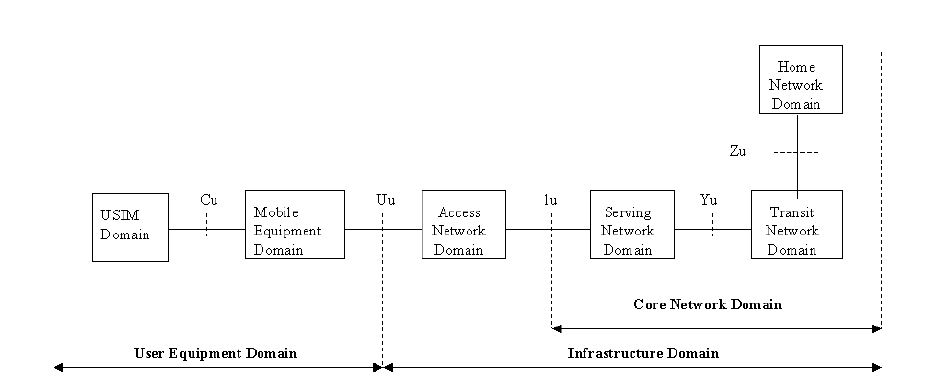
\includegraphics[width=\linewidth]{Kapitel/3G/Grafiken/Domains.jpg}
\captionof{figure}{Übersicht Domains~\cite{3G.1}}
\label{fig:vorlage.vorlesungssaal}
\end{Figure}
 
Die AND wird bei UMTS durch UMTS Terrestrial Radio Access Network (UTRAN) umgesetzt und ermöglicht die Ankopplung eines Mobiltelefons an das Core Network. Der Aufbau von UTRAN besteht aus mehreren Radio Network Subsystems (RNS). Diese werden jeweils von einem Radio Network Controller (RNC) gesteuert. Hierbei hat der RNC mehrere Aufgaben, wie beispielsweise die Ver – und Entschlüsslung, die Staukontrolle sowie weitere Verwaltungsaufgaben. Ein solcher RNC verwaltetet hierbei einen oder mehrere Node B (Basisstationen), wobei eine solche Node B eine oder mehrere Antennen Steuert. Die Antennenanzahl bedingt dann wiederum das Aufspannen einer oder mehrer Funkzellen.

Die Core Network Domain (CND) ist auch als Kernnetz bekannt und ermöglicht Verbindungen in das eigene Netz oder in andere Systeme. Hierbei wird CND nochmals in Serving Network Domain (SND), Home Network Domain (HND) und Transit Network Domain (TND) aufgeteilt. In diesen Bereichen wird das Routing, die Lokalisierung, das Roaming, das Billing und das Charging umgesetzt. Weiterhin wird das Kernnetz in zwei weitere Bereiche eingeteilt. Einmal in die Circuit Swiched Domain, welche der Leitungsvermittlung dient und andererseits in die Packet Switched Domain, diese dient zur Paketvermittlung. Diese Unterscheidung ist bedingt durch die Dienste, welche mittelst des Dienstes genutzt werden. So sind Datendienste, wie das Verschicken eines Bildes auf die Paketvermittlung, angewiesen und Telefongespräche auf eine Leitungsvermittlung.  Diese Abtrennungen der beiden Domains sind oftmals nur Modellhaft, die tatsächliche Umsetzung besteht lediglich nur aus einem Bauteil. Eine weitere Aufgabe des Kernnetzes ist die Verwaltung von mehreren Mobile-service Switching Centre (MSC) beziehungsweise Serving GPRS Support Nodes (SGSN) in den einzelnen RNS. Hierbei verwaltet nun jede MSC zusätzlich eine Home Location Register (HLR), welches die Nutzerdaten beheimatet und ein Visitor Location Register (VLR). Der Abbildung 2 kann ein solcher modellhafter Aufbau entnommen werden.

\begin{Figure}
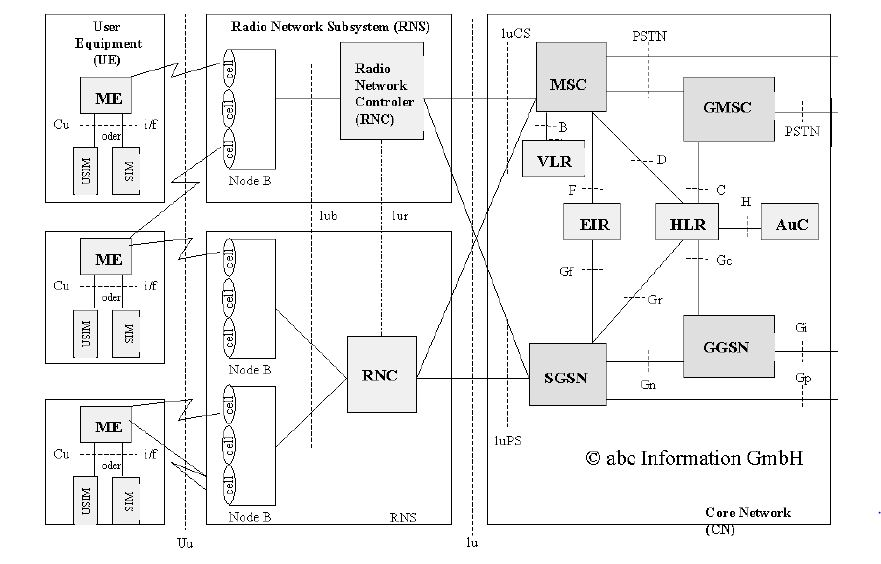
\includegraphics[width=\linewidth]{Kapitel/3G/Grafiken/Architektur.jpg}
\captionof{figure}{Architektur UMTS ~\cite{3G.1}}
\label{fig:vorlage.vorlesungssaal}
\end{Figure}

Die Direct-Sequence-(DS)-CDMA-Technik macht nun großen Unterschied zwischen GSM und UMTS im Bereich der Funkschnittstelle aus. Hierbei steht CDMA für ein Codemultiplexverfahren, welches einen Datenstrom mit einer Chipping-Sequenz multipliziert. Der so erzeugt Code wird im Anschluss daran abhängig von dem Netzbetreiber über einem Frequenzband gespreizt, üblich sind hierbei Bandbreiten zwischen 4,4 MHz und 5 MHz. Durch die auf Spreizung können Störungen verringert werden und weiterhin bei einer bestimmten Spreizung eine Trennung des Signals von Hintergrundgeräuschen, ohne Kenntnisse des Codes, ausgeschlossen werden.~\cite{3G.1, 3G.4}


\subsubsection*{HSDPA}
HSDPA wurde als Weiterentwicklung von UMTS mit dem 5. Release eingeführt.  Der große Vorteil von HSDPA besteht darin das es neben UMTS koexistieren kann und auch auf der Technologie von UMTS aufbaut. Eine Erneuerung war die verkürzte Latenzzeit von 100 ms. Weiterhin kann HSDPA nun die Leistung einer Funkzelle dauerhaft nutzen, was durch einen neuen Funkkanal erreicht wurde. Die Steuerung des Nutzkanals übernimmt hierbei der High Speed Dedicated Physical Control Channel (HS-SCCH). Durch High Speed Downlink Shared Channel (HS-DSCH) und High Speed Physical Shared Channel (HS-PSCH) konnte die verbesserte Übertragungsgeschwindigkeit erreicht werden. Auch das Short Transmission Time Interval (STTI), die Zeit die die Übertragung eines Datenpakets benötigt, wurde um ein Fünftel verringert und beträgt somit 2 ms.  Auch das Multiplexing würde bei HSDPA durch die Kombination von CDMA und TDMA (Zeitmultiplexing) verbessert. Durch die Einteilung der Zeitachse in mehre Bereiche können jedem Nutzer ein Zeitbereich bereitgestellt werden. Dieser Bereich hat dann die STTI-Zeitdauer.~\cite{3G.1, 3G.3}

\subsection*{Einsatz}

Nachdem nun der theoretische Aufbau bekannt ist, folgt eine Erläuterung zum Aufbau einer Sprach- oder Datenverbindung. Zu Beginn muss jedes Mobiletelefon eine SIM-Karte besitzen und sich in einem HLR registrieren. Im nächsten Schritt muss eine Verbindung zu einer Basisstation aufgebaut werden. Dieser Wunsch nach dem Aufbau einer Verbindung leitet die Basisstation weiter zu dem RNC, der diese ebenfalls an den MSC weiter gibt. Dort angekommen ordnet der MSC die Telefonnummer dem Nutzer zu und durch Routing kann nun das HLR angesprochen werden. Im Anschluss daran wird die Position bzw. die Zelle in der sich das Mobilfunkgerät eingewählt hat dem HLR übermittelt. Der Ort wird im HLR vermerkt und es werden ein Teil der Nutzerdaten an das VLR der aufrufenden MSC gesendet. Nun wird das Mobiltelefon authentifiziert und daraufhin kann ein Telefongespräch mit diesem Gerät geführt werden. Dazu muss nun erneute der Wunsch durch die Basisstation an die RNC und im Anschluss da-

\end{multicols}
\newpage
\section*{Historische Entwicklung}
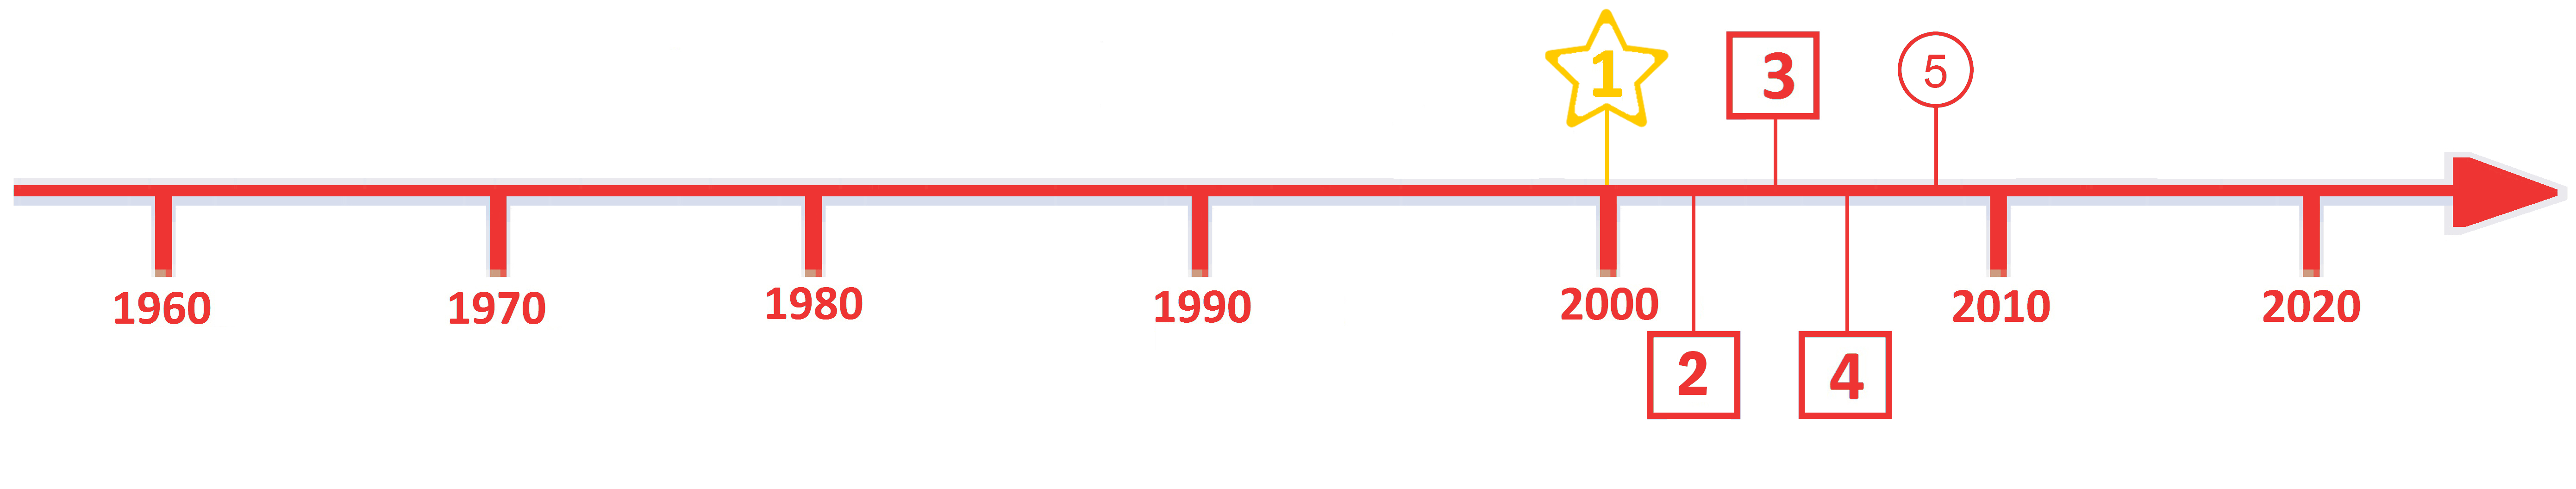
\includegraphics[width=\textwidth]{Kapitel/3G/Grafiken/Zeitstrahl}
\par
\noindent
\begin{tabular}{|p{1 cm}|p{3 cm}|p{13.55 cm}|}
	\hline
	Nummer & Datum & Entwicklungsschritte ~\cite{3G.2}\\
	\hline
	1 & 2000 & Einführung von UMTS in den deutschen Markt\\
	\hline
	2 & 2004 & Einführung von UMTS fähigen Endgeräten\\
	\hline
	3 & 2006 & Einführung von HSDPA in den deutschen Markt\\
	\hline
	4 & ab 2007 & Hohe Netzabdeckung von UMTS und HSDPA innerhalb von Deutschland \\
	\hline
\end{tabular}
\par
\begin{multicols}{3}


ran an die MSC weitergeleitet werden. Soll nun ein anderes Mobiltelefon angerufen werden, wird dieses durch die HLR aufgerufen, denn dort sind Positionsdaten gespeichert. Daraufhin kann die Zelle angesprochen werden in dem sich das Mobiltelefon befindet und der Anruf kann getätigt werden. 
Durch den Dezentralen Aufbau dieses Netzes kann ein Gesamtausfall vermieden werden da höchstens Teilgebiete des Mobilfunkproviders ausfallen können. ~\cite{3G.1}

\subsection*{Anbieter und Gremien}
Wie bereits erwähnt lag der Ausbau dieser Netze an den Firmen, welche als erstes Lizenzen für UMTS ergattern konnten. Die Firmen T-Mobile Deutschland GmbH, Vodafone D2 GmbH, MobilCom Multimedia GmbH, Auditorium Investments Germany S.à.r.l. (später umformiert in E-plus 3G Luxemburg S.à.r.l.), O2 und Group 3G (ein Konsortium aus der spanischen Telefónica und der finnischen Sonera)erhielten diese zu Beginn.  Doch in den Folgejahren geben die Firmen MobilCom Multimedia GmbH und Group 3G ihre Lizenzen wieder ab.
Die HSDPA Netzanbieter von Deutschland sind T-Mobile, Vodafone, o2 und E-Plus. Alle bekannten Anbieter von 3G Tarifen nutzen das Netz einer dieser Provider. 
~\cite{3G.1, 3G.2}

\subsection*{Ausblick}
Der nächste Schritt in der Evolutionären Entwicklung des mobilen Internets ist 4G oder auch LTE (Long Term Evolution). Mitte August des Jahres 2010 wurde in Deutschland der erste LTE-Sendemast errichtet. Aber nahere Erläuterungen zu LTE finden Sie im folgenden Artikel ~\cite{3G.2}.


\printbibliography[segment=8,heading=subbibliography]
\end{multicols}



\newpage
